% !TeX spellcheck = en_US
% !TeX root = ./0_article.tex

\section{Introduction}
%\IEEEPARstart{S}{everal} researches have studied Body Biasing Injection (BBI) in the past few years.
%While this injection method had been \textcolor{orange}{paused/forgotten} for a few years, it has recently regained some interest.
%Among the latest studies, a modeling and simulation flow has been proposed, alongside better platforms allowing to achieve greater reproducibility and a deeper analysis of the mechanisms at works in digital integrated circuits subjected to BBI.
%In addition to that

%	\subsection{Context}
	\IEEEPARstart{W}{hen} working with cybersecurity, specifically with hardware security, various fault injection methods are often considered.
	One can point out Electromagnetic Fault Injection (EMFI) \cite{mathieuEMFIFirst, mathieuEMFI}, Laser Fault Injection (LFI) \cite{lfiFaultModel}, or Body Biasing Injection (BBI) \cite{bbiOrigin}, not to cite them all.
	The current work is dedicated in studying Body Biasing Injection.

	Nowadays, electronic devices are found in every economic sector, and very often they manipulate sensitive data, such as in bank transactions, Internet of Things (IoT) devices, or smartphones.
	To ensure data authenticity, these devices embed cryptographic algorithms.
	While theoretically secure, once implemented on actual devices, these algorithms become fallible, leaking manipulated data, in addition to being sensitive to external disturbances.

	\subsection{Fault injection objectives}
		Fault injection methods are set up to perform various malicious manipulation on integrated circuits, such as:
		\begin{itemize}
			\item Denial of service (DoS) \textrightarrow\ Stop circuit operation and the related services;
			\item Verification bypass \textrightarrow\ Modify data on the fly to fake authenticity (e.g. to bypass bootloader security);
			\item Confidential data extraction \textrightarrow\ Modify data to perform differential fault analysis.
		\end{itemize}

	\subsection{BBI in the state-of-the-art}
		When compared to EMFI, BBI has a smaller state-of-the-art, whether in the amount of scientific papers published or in the amount of industrial platforms proposed.
		Currently, there are ten main works lingering on BBI \cite{bbiOrigin, bbiSecond, bbiThird, bbiColin,japbbi, japbbi2, mybbiCosade, mybbiFdtc2022, mybbifdtc2023, colinFdtc2023}.
		Each one of them made a unique contribution for a better understanding of BBI.

		The first one \cite{bbiOrigin} introduced the technique and presented a Bellcore attack on the targeted IC.
		Then, one year later, another work \cite{bbiSecond} further studied the method, followed by a third work three years later \cite{bbiThird}, introducing an advanced test bench to work and perform attacks with BBI.

		However, there are still unanswered questions, and the current works aims at bringing more answers thanks to previous and new data.

		Before introducing the present work, let us eventually analyze the industrial platforms proposed by various manufacturers and introduce our own test platform.
		We can distinguish three major actors proposing BBI related products:
		\begin{itemize}
			\item Langer EMV-Technik;
			\item Riscure;
			\item NewAE Technology.
		\end{itemize}

		% !TeX spellcheck = en_US
% !TeX root = ./0_article.tex

\begin{figure}
	\centering
	\subfloat[][Langer]{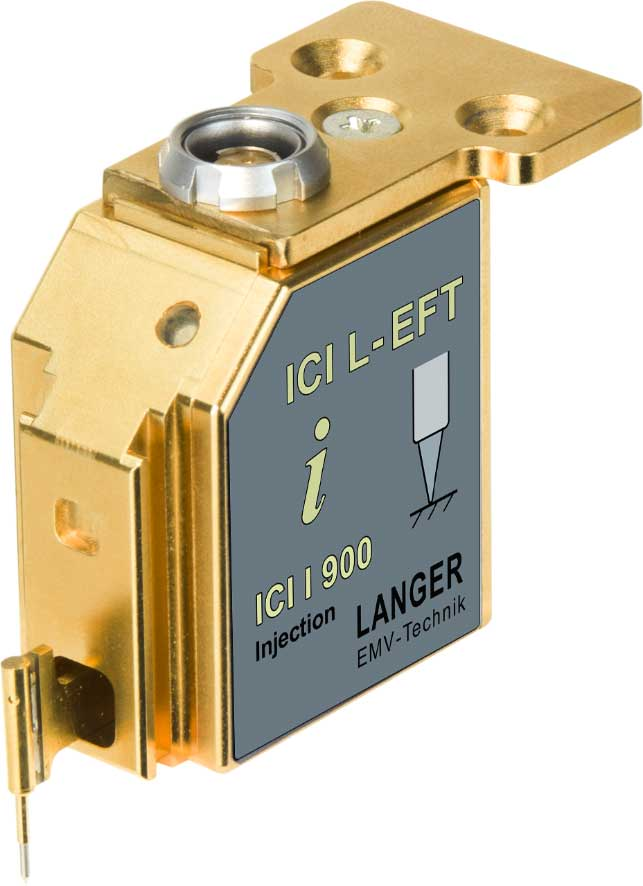
\includegraphics[width=0.2\columnwidth]{./figures/langerBBI.jpg}}
	\hspace{0.1\columnwidth}
	\subfloat[][Riscure]{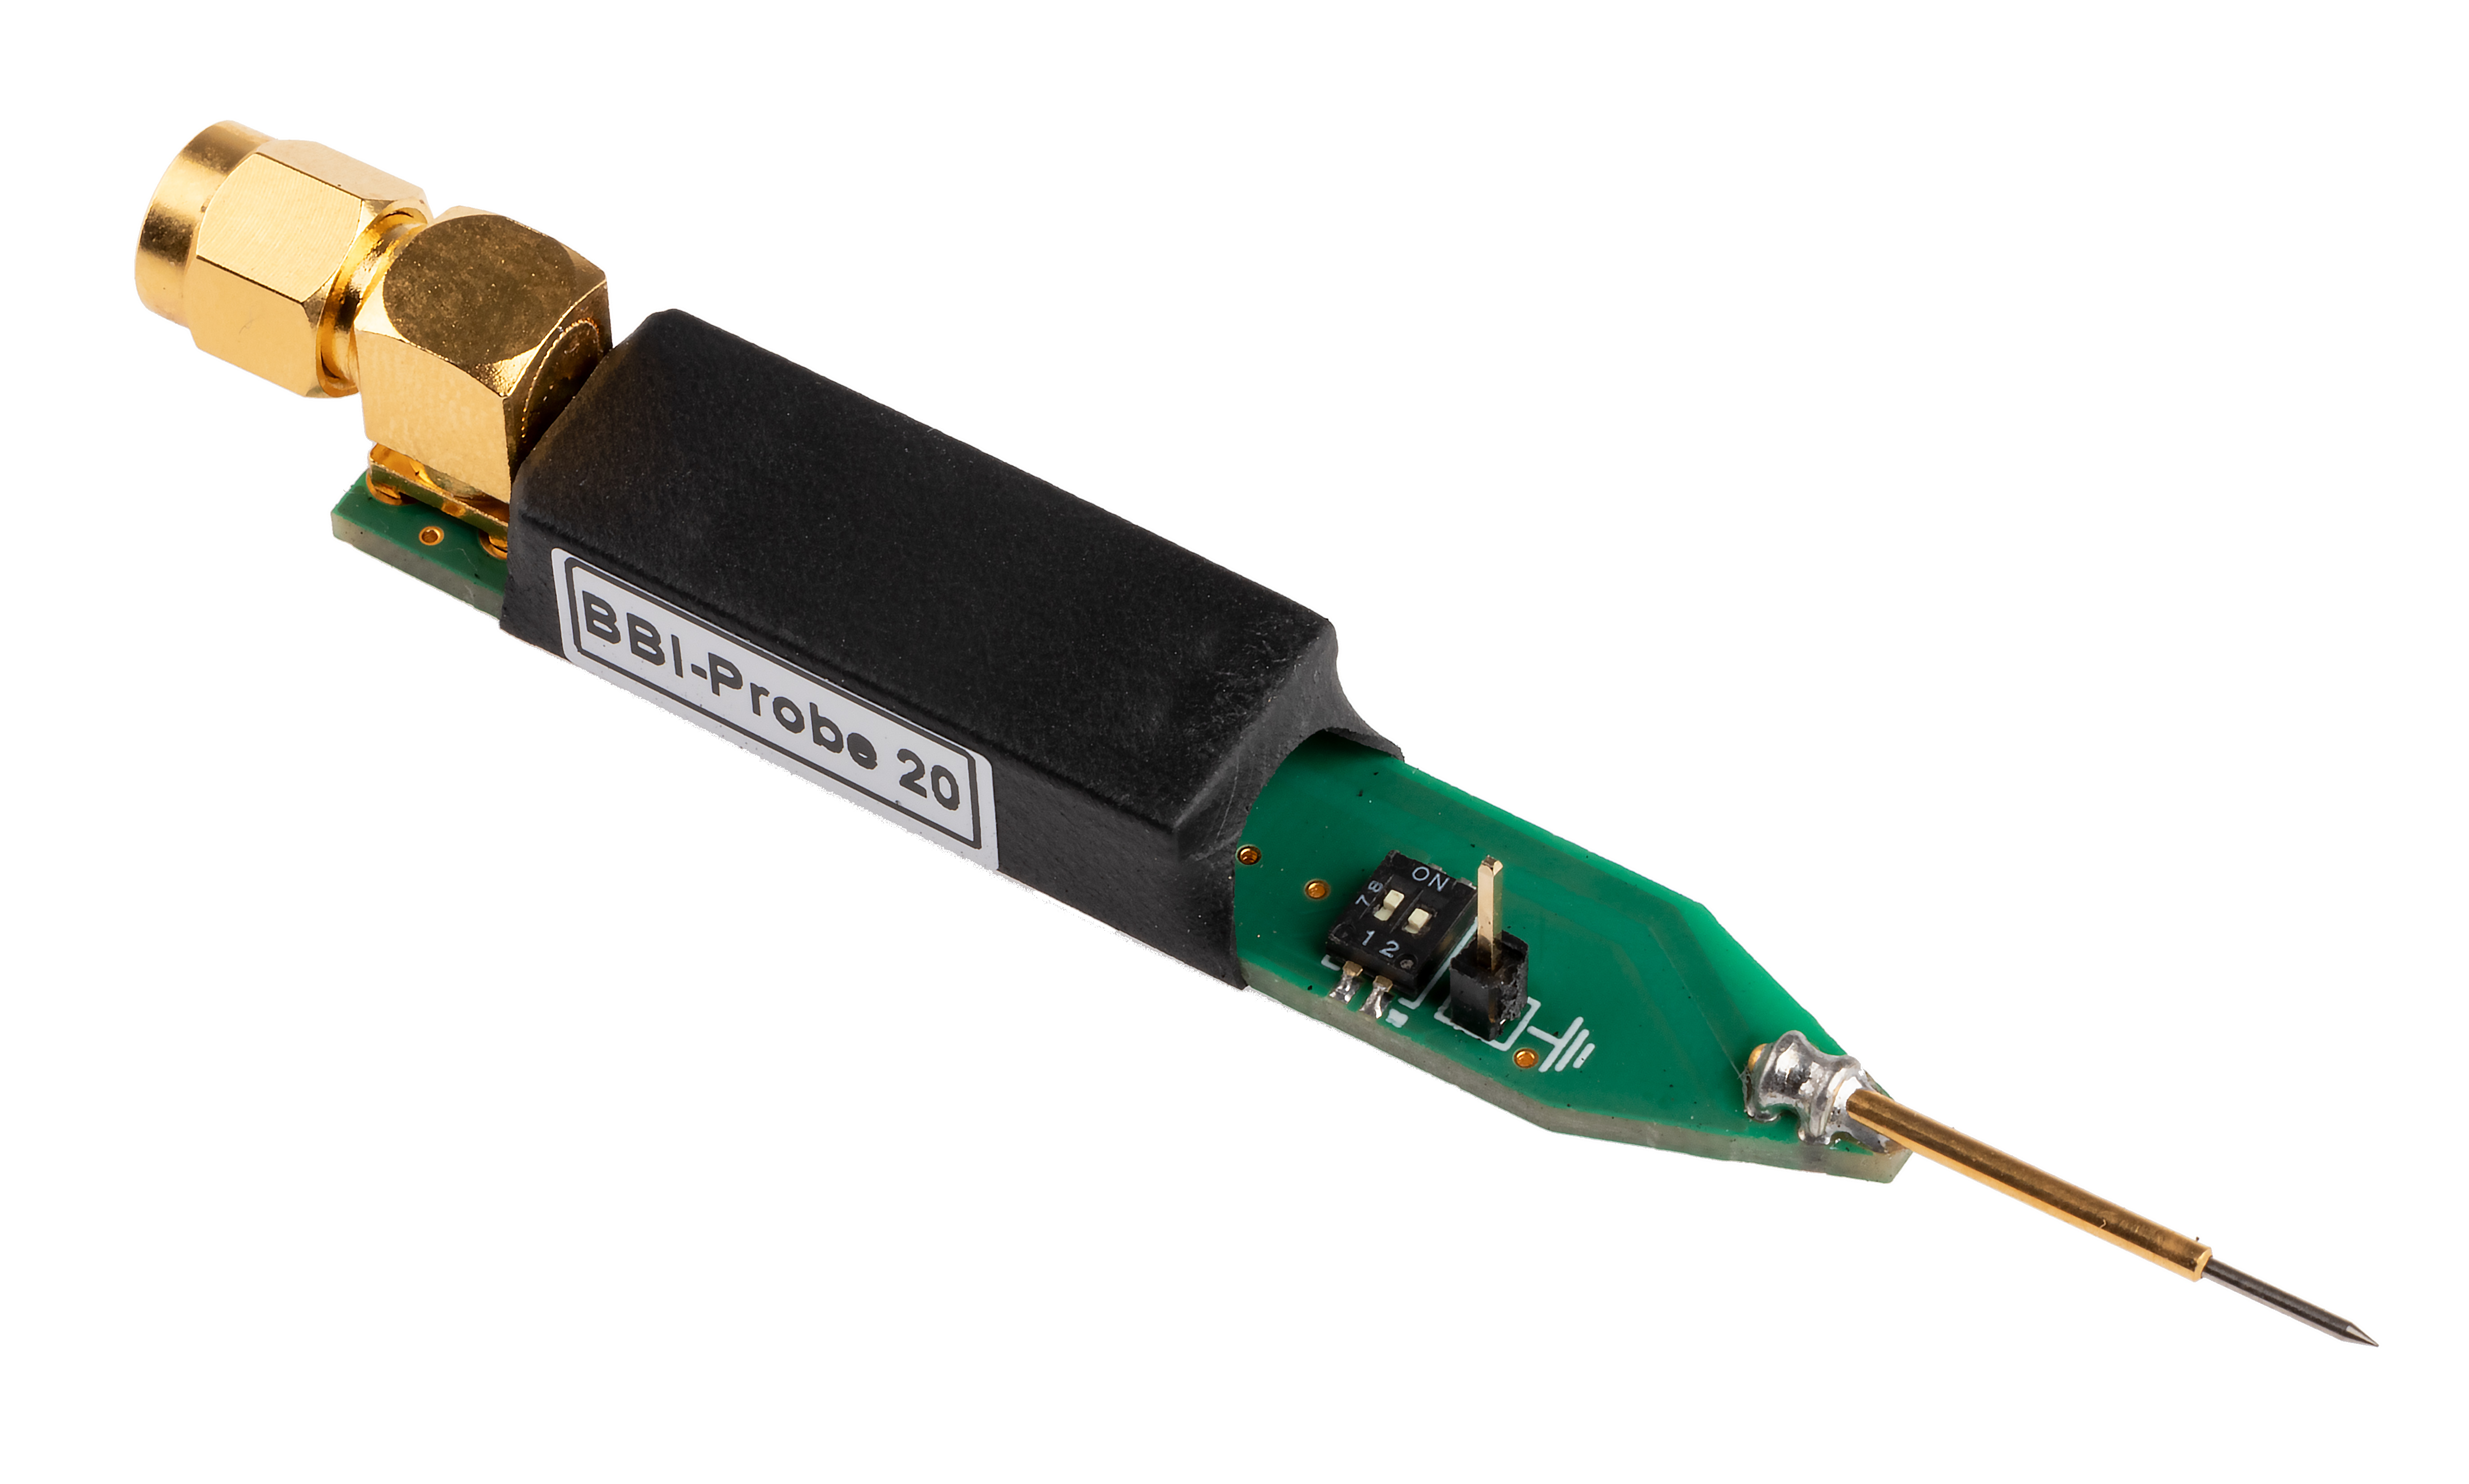
\includegraphics[width=0.425\columnwidth]{./figures/em-fi-bbi-probe-20-black.jpg}}
	\caption{Langer and Riscure BBI probes.}
	\label{riscure_langer}
\end{figure}
		\subsubsection{Langer EMV-Technik platform}
			The German society Langer EMV-Technik proposes an all-in-one and ready-to-use BBI platform composed of two hardware tools:
			\begin{itemize}
				\item A current pulse generator with a metal needle, shown in left in Fig. \ref{riscure_langer};
				\item A general controller called "Burst Power Station", combining a power supply, control and monitor tool and a software.
			\end{itemize}

	\subsection{BBI interrogations}
		With all the work in the state-of-the-art in mind, there are still remaining questions unanswered about BBI, such as:
		\begin{itemize}
			\item What is the spatial resolution of BBI?
			\item What is the time resolution of BBI?
			\item Is thinning the substrate useful in any way?
			\item How BBI induced faults occur?
			\item How to properly model BBI?
		\end{itemize}
